
\section{What is quantum computing?}

\begin{frame}[plain]
\frametitle{A few  citations}

\begin{quotation}{Niels Bohr - }
    Everything we call real is made of things that cannot be regarded as real. If quantum mechanics hasn't profoundly 
    shocked you, you haven't understood it yet.
\end{quotation}

\begin{quotation}{Niels Bohr - }
    Everything we call real is made of things that cannot be regarded as real.
\end{quotation}

\begin{quotation}{Richard Feynmann - }
    If you thought that science was certain - well, that is just an error on your part.
\end{quotation}

\begin{quotation}{Richard Feynmann - }
    I think I can safely say that nobody really understands quantum mechanics
\end{quotation}

\begin{quotation}{Richard Feynmann, 1982 - }
    Nature isn’t classical, dammit, and if you want to make a simulation of nature, you better 	
    make it quantum mechanical
\end{quotation}

\begin{quotation}{Albert Einstein - }
    If you can't explain it simply, you don't understand it well enough
\end{quotation}

\end{frame}

\begin{frame}{What is a computer?}
\begin{tikzpicture}[remember picture, overlay]
\node[left] at (current page.east) 
{
    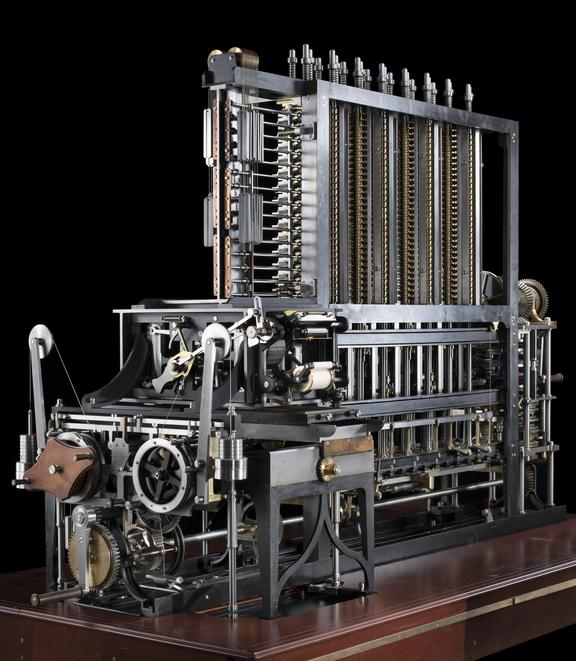
\includegraphics[width=0.25\textwidth]{images/babbage2.jpg}
};
\end{tikzpicture}    
From Wiktionnary, \begin{quotation}
   A computer is a machine that can be programmed to automatically carry out sequences of arithmetic or logical operations (computation). 
\end{quotation}
Several machines are illustrations of this concept:
\begin{itemize}
    \item the \textit{differences engine} by Lord Babbage, fully mechanical,
    \item computers based on electronics, based on Maxwell's theory (and transistors)
\end{itemize}
A Quantum computer is,
\begin{itemize}
    \item a logicam evolution of the concept, this time quantum mechanics is sued to build computatiion devices
\end{itemize}

\end{frame}

\begin{frame}[plain]
\frametitle{Quantum Computing is not really recent}
Le \textit{Quentum Computing} is born in the 80s
\begin{itemize}
   \item a first conferenceabout QC occurend at MIT in 1981
   \item Many theorical studies are made about QC, leading to revolutionnary algorithms
   \begin{itemize}
       \item Shor Algorithm, 1994
       \item Grover Algorithm, 1996
   \end{itemize}
\end{itemize}

QC has very concrete theorical basements
\begin{itemize}
    \item in physics (quantum physics, statistical physics)
    \item in mathematics (linear algebra, hermitian algebra)
\end{itemize}


Real "Quantum Computers" exists for a few years only. 

\end{frame}

\begin{frame}[plain]
\frametitle{Links between Quantum Compurting and Quantum Physics}
\textit{Quantum Computing} is a new paradigm based on Quantum Physics phenomenons:
\begin{enumerate}
    \item superposition,
        \begin{itemize}
            \item QC introduces a \textit{kind of} material paralellism
        \end{itemize}
    \item entanglement,
         \begin{itemize}
            \item couples simpler system in order to build larger systems
         \end{itemize}
    \item interferences,
        \begin{itemize}
            \item make it possible to build unitary operators and measure quantum physics observables
         \end{itemize}
\end{enumerate}
\end{frame}

\begin{frame}{The first quantum revolution}
    Quantum Physics is already there in your everyday life.  
    \begin{itemize}
        \item medicine : MRI, magnetic resonance imaging.,
        \item electronics : Transistors based on tunnel effect, LED,
        \item lasers,
        \item LCD screens,
        \item  photovoltaïcs : photon/matter interaction.
    \end{itemize}
\end{frame}

\begin{frame}{QC and the second quantum revolution}
Quantum Computing belong to the second quantum revolution\\[0.5cm]

 \textbf{QPU}s start appearing on the market. \\[0.5cm]

Several steps are identified
\begin{itemize}
    \item NISQ : \textbf{N}oisy \textbf{I}ntermediate \textbf{S}cale \textbf{Q}uantum
    \item FTQC : \textbf{F}ault \textbf{T}olerant \textbf{Q}uantum \textbf{Q}uantum
    \item LSQ : \textbf{L}arge \textbf{S}cale \textbf{Q}uantum
\end{itemize}
We currently are in the NISQ era. 

\begin{tikzpicture}[remember picture, overlay]
\node[left] at (current page.east) 
{
    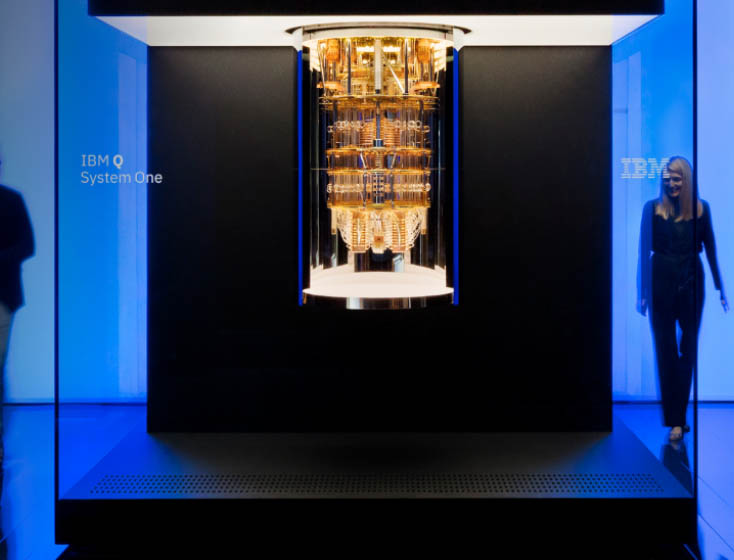
\includegraphics[width=0.25\textwidth]{images/QPU-IBM.jpg}
};
\end{tikzpicture}

\end{frame}

\begin{frame}{What Quantum Computing is not}
QC will never replace HPC
\begin{itemize}
    \item QPUs buold a new HPC paradigm, such as GPUs.
    \item QC is a new weapon in the HPC's armory
\end{itemize}

Beware the "Quantul Hype"!!!!
\begin{itemize}
    \item advertissements, often far from reality
    \item fuzzy articles in general purpose newpapers, 
    \item QC is not "doing $2^n$ computations at the same time", exponential parallelism exists but it does not 
    occur everytime.
    \item  QC  is good to ccaracterize a global property of a known problem
    \begin{itemize}
        \item periodicity of an integer function (Shor)
        \item walking a graph (quantum walks)
        \item locating optima of a quadratic function (QUBO)
    \end{itemize}
\end{itemize}
\end{frame}